\iffalse
\title{2011-XE}
\author{EE24BTECH11020 -  Ellanti Rohith}
\section{xe}
\chapter{2011}
\fi
   \item A certain fluid flow is influenced by density $\rho$, angular velocity $\omega$, dynamic viscosity $\mu$, and a characteristic length $L$. A relevant non-dimensional parameter will be \hfill{[GATE 2011]}
    \begin{multicols}{4}
    \begin{enumerate}
        \item $\rho \omega \mu / L^2$
        \item $\rho \omega L^2 / \mu$
        \item $\rho \mu L^2$
        \item $\rho \omega \mu L$
    \end{enumerate}
    \end{multicols}
    
\item The drags due to potential flow past a cylinder of diameter $D$ cm and a slender airfoil of chord length $D$ cm are compared. Assuming unit depth for both bodies, which one of the following would be \textbf{TRUE}?\hfill{[GATE 2011]}
    
    \begin{enumerate}
        \item The drag on the cylinder is greater
        \item The drag on the airfoil is greater
        \item Both the drags are equal
        \item Additional data is needed to compare the drags
    \end{enumerate}
        
    \item For a fully developed flow between two parallel flat plates, the velocity gradient at a point is found to be $1000 \, \text{s}^{-1}$. If the density of the fluid is $880 \, \text{kg/m}^3$ and the kinematic viscosity of the fluid is $7.4 \times 10^{-7} \, \text{m}^2/\text{s}$, the shear stress at the same point is approximately\hfill{[GATE 2011]}
    \begin{multicols}{4}
    \begin{enumerate}
        \item 0 Pa
        \item 1.30 Pa
        \item 0.32 Pa
        \item 0.65 Pa
    \end{enumerate}
    \end{multicols}
    
    \item An open channel flow is to be simulated in the laboratory. For this purpose, a 1:25 scale model is constructed. If the flow velocity in the prototype is $5  \text{ m/s}$, for dynamic similarity the model should have a flow velocity of\hfill{[GATE 2011]}
    \begin{multicols}{4}
    \begin{enumerate}
        \item $5  \text{ m/s}$
        \item $1  \text{ m/s}$
        \item $125  \text{ m/s}$
        \item $25  \text{ m/s}$
    \end{enumerate}
    \end{multicols}

\textbf{Q.10 - Q.22 carry two marks each.}

\item A pitot-static probe is inserted in an air flow. A manometer connected to this probe having Hg as the manometric fluid shows a difference of $30 \, \text{mm}$. Assume a probe factor of 1. Assuming $\rho_{\text{air}} = 1.23 \, \text{kg/m}^3$, $\rho_{\text{Hg}} = 13600 \, \text{kg/m}^3$ and $g = 10 \, \text{m/s}^2$, the speed of the air flow is approximately\hfill{[GATE 2011]}
  \begin{multicols}{4}
    \begin{enumerate}
        \item $66.5 \text{ m/s}$
        \item $76.5 \text{ m/s}$
        \item $81.5 \text{ m/s}$
        \item $92.5 \text{ m/s}$
    \end{enumerate}
    \end{multicols}

\item Consider an L-shaped gate with water level above the hinge as shown. At approximately what height $D$ of the water level will the gate open? Neglect the mass of the gate. Assume $g = 10 \, \text{m/s}^2$.

\begin{center}


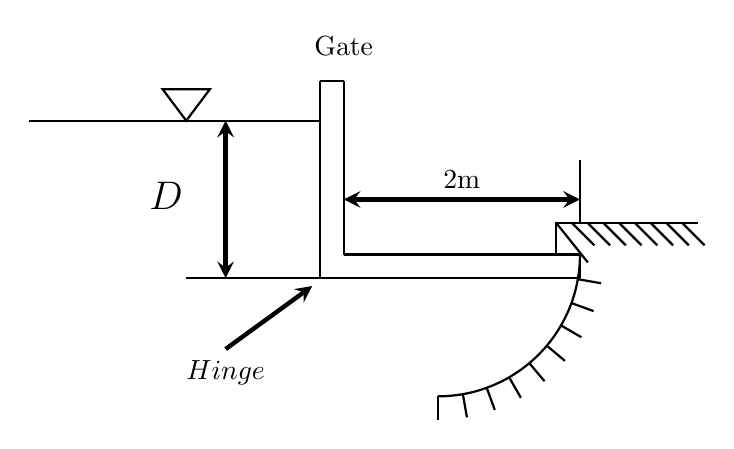
\begin{tikzpicture}
   
    \draw[thick] (-4,-1) -- (-0.3,-1);

   
    \draw[<->,ultra thick,>=stealth] (-1.5,-1) -- (-1.5,-3);\draw[->,ultra thick,>=stealth] (-1.5,-3.9) -- (-0.4,-3.1);\node at (-1.5,-4.2) { $Hinge$};  \draw[thick](-2,-1)--(-2.3,-0.6)--(-1.7,-0.6) -- cycle;
    \node[left] at (-1.92,-1.95) {\Large $D$};

    

    \draw[thick] (0,-0.5) -- (0,-2.7);         
    \draw[thick] (-2,-3) -- (3,-3);           
    \draw[thick] (-0.3,-0.5) -- (-0.3,-3);     
    \draw[thick] (3,-2.7) -- (-0,-2.7);   \draw[thick] (3,-2.7) -- (3,-3);    

    
    \draw[<->,ultra thick,>=stealth] (0,-2) -- (3,-2);
    \node at (1.5,-1.75) {2m};
   

    \draw[thick] (0,-0.5)--(-0.3,-0.5);

    
    \draw[thick] (3,-2.7) arc[start angle=0, end angle=-90, radius=1.8];
\foreach \angle in {-10,-20,-30,-40,-50,-60,-70,-80,-90} {
    \draw[thick] 
        (1.2,-2.7) ++(\angle:1.8) -- ++(\angle:0.3);
}
    \draw[thick] (2.7,-2.7)--(2.7,-2.3) -- (4.5,-2.3);
    \foreach \x in {2.9,3.1,3.3,3.5,3.7,3.9,4.1,4.3} {
        \draw[thick] (\x,-2.3) -- ++(-45:0.4);
    }\draw[thick] (2.7,-2.3)--(3.1,-2.8);
    \draw[thick] (3,-2.3)--(3,-1.5);
     \node[above] at (0,-0.3) {Gate};
\end{tikzpicture}
\end{center}
\hfill{[GATE 2011]}
\begin{multicols}{4}
\begin{enumerate}
    \item 3.46 m
    \item 4.36 m
    \item 6.43 m
    \item 5.36 m
\end{enumerate}
\end{multicols}


\item When a large tank containing water is placed on a weighing scale, a reading of 10000 N is obtained. The tank is fitted with an outlet pipe and a valve as shown. When the valve is opened, a jet of water with a velocity of 10 m/s issues out in the vertically upward direction. The diameter of the outlet pipe is 10 cm. Determine approximately the reading on the weighing scale at the instant the valve is opened and the water jet issues out. Density of water is 1000 kg/m$^3$.

\begin{center}
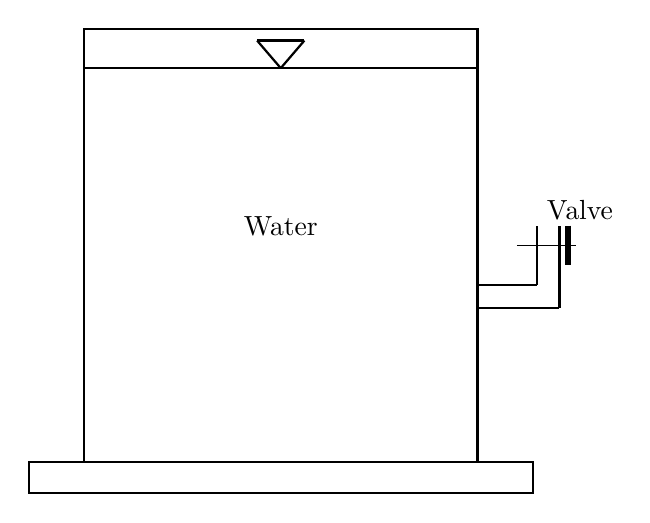
\begin{tikzpicture}
    
    \draw[thick] (-1,0) rectangle (4,5);
     \draw[thick] (-1,5) rectangle (4,5.5);
    \draw[thick] (-1.7,0) rectangle (4.7,-0.4);
    \node at (1.5,3) {Water};
    \node at (5.3,3.2) {Valve};

    
    
    
    \draw[thick] (4,2.25) -- (4.75,2.25);
    \draw[thick] (4.75,2.25) -- (4.75,3);  \draw (4.5,2.75) -- (5.25,2.75);  \draw[line width=2pt] (5.15,3) -- (5.15,2.5); 
    \draw[thick] (4,1.95) -- (5.04,1.95);
    \draw[thick] (5.04,1.95) -- (5.04,3); 
    
    \draw[thick] (1.5,5) -- (1.2,5.35);
    \draw[thick] (1.5,5) -- (1.8,5.35);
    \draw[thick] (1.2,5.35) -- (1.8,5.35); ;
\end{tikzpicture}
\end{center}
\hfill{[GATE 2011]}
\begin{multicols}{4}
\begin{enumerate}
    \item 9215 N
    \item 10000 N
    \item 10785 N
    \item 12500 N
\end{enumerate}
\end{multicols}


\item A fluid with a volumetric flow rate of 5 m$^3$/s enters the nozzle shown below. The cross-sectional area varies with $x$ as $A(x) = \frac{1}{(1 + x^2)}$. Assuming that the flow is parallel and uniform at each cross-section, the acceleration at any point in the nozzle is given by

\begin{center}
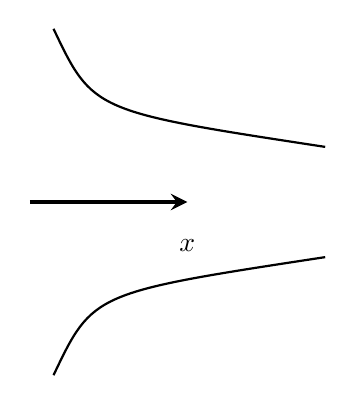
\begin{tikzpicture}
   
    \draw[thick] (-1.7,2.5) .. controls (-1.2,1.45) .. (1.75,1); 
    \draw[thick] (-1.7,-1.9) .. controls (-1.2,-0.85) .. (1.75,-0.4);
    \draw[->, ultra thick, >=stealth] (-2,0.3) -- (0,0.3); 
    \node[below] at (0,-0.05) {$x$};
\end{tikzpicture}
\end{center}
\hfill{[GATE 2011]}
\begin{multicols}{4}
\begin{enumerate}
    \item 50($x + x^3$)
    \item 50($1 + x^2$)
    \item 0
    \item 50($x^2 + x^3$)
\end{enumerate}
\end{multicols}


\item Consider fully developed flow of water in a pipe of diameter 2 cm. The average velocity of the flow is 2 m/s. The viscosity of the water is 10$^{-3}$ kg/m$\cdot$s and the density is 1000 kg/m$^3$. The friction factor can be calculated using $f = 64 / \text{Re}$ for laminar flows and $f = 0.3164 / \text{Re}^{0.25}$ for turbulent flows. The pressure drop over a length of 0.5 m is
\hfill{[GATE 2011]}
\begin{multicols}{4}
\begin{enumerate}
    \item 0.08 Pa
    \item 325 Pa
    \item 1115 Pa
    \item 9875 Pa
\end{enumerate}
\end{multicols}
\item Consider a steady, fully developed flow in a horizontal pipe of diameter $D$. Over a section of length $L$ of this pipe, a pressure drop of $\Delta p$ is observed. The average wall shear stress over this section is\hfill{[GATE 2011]}
    \begin{multicols}{4}
        \begin{enumerate}
            \item $\frac{\Delta p D}{4L}$
            \item $\frac{\Delta p D}{2L}$
            \item $\frac{\Delta p \pi L}{2D}$
            \item $\frac{\Delta p \pi L}{4D}$
        \end{enumerate}
    \end{multicols}
    
\item In an inviscid incompressible flow, the velocity field is given by $\vec{V} = x\hat{i} + y\hat{j}$ m/s and the body force per unit mass is given by $\vec{g} = -10\hat{k}  \text{ m/s}^2$. The pressure at the point $(0, 0, 0)$ is 101 Pa. Assuming that the density of the fluid is $1 \, \text{kg/m}^3$, the pressure at the point $(1, 1, 1)$ for this flow is\hfill{[GATE 2011]}
    \begin{multicols}{4}
        \begin{enumerate}
            \item $100 \, \text{Pa}$
            \item $105 \, \text{Pa}$
            \item $95 \, \text{Pa}$
            \item $90 \, \text{Pa}$
        \end{enumerate}
    \end{multicols}
    


\textbf{Common Data Questions}

\textbf{Common Data for Questions 17 and 18:}

A two-dimensional rectangular water jet of velocity $10 \, \text{m/s}$ and area $5 \, \text{cm}^2$ impinges normal to a flat plate and splits symmetrically into two half jets, each of area $2.5 \, \text{cm}^2$ as shown. Assume steady flow and neglect viscous effects and the weight of the plate and the water. Density of water is $1000 \, \text{kg/m}^3$.

\begin{centering}
    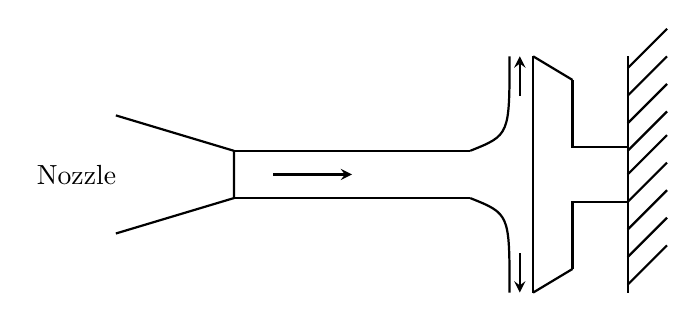
\begin{tikzpicture}
  
   \draw[thick] 
    (1, 0.3) -- (-0.5, 0.75)
    (1, 0.3) -- (1, -0.3) -- (-0.5, -0.75);
\draw[thick]
    (1, 0.3) -- (4, 0.3) 
    (1, -0.3) -- (4, -0.3); 

\draw[->, thick, >=stealth]
    (1.5, 0) -- (2.5, 0);

    \draw[->, thick, >=stealth] (4.63, 1) -- (4.63, 1.5); 
    \draw[->, thick, >=stealth] (4.63, -1) -- (4.63, -1.5); 
    \node at (-1, 0) {Nozzle}; 
     \draw[thick] (4,0.3) .. controls (4.5,0.5) .. (4.5,1.5);
     \draw[thick] (4,-0.3) .. controls (4.5,-0.5) .. (4.5,-1.5);
   
    \draw[thick] (5.3, 1.2) -- (5.3, 0.35)--(6,0.35);  \draw[thick] (5.3, -1.2) -- (4.8, -1.5); \draw[thick] (5.3, 1.2) -- (4.8, 1.5); 
    \draw[thick] (4.8, -1.5) -- (4.8, 1.5); 
   \draw[thick] (5.3, -1.2) -- (5.3, -0.35)--(6,-0.35); 

  
    \foreach \y in {-1.4,-1.05,-0.7,-0.35, 0, 0.30, 0.65,1,1.35} {
        \draw[thick] (6, \y) -- (6.5, \y + 0.5);
    }
    \draw[thick] (6, 1.5) -- (6, -1.5); 
    \end{tikzpicture}

\end{centering}
    




\item After splitting, the velocity of the upward half-jet along the plate is\hfill{[GATE 2011]}
    \begin{multicols}{4}
        \begin{enumerate}
            \item $5  \text{ m/s}$
            \item $7.5  \text{ m/s}$
            \item $2.5  \text{ m/s}$
            \item $10  \text{ m/s}$
        \end{enumerate}
    \end{multicols}
    
\item The magnitude of the reaction force at the wall is\hfill{[GATE 2011]}
    \begin{multicols}{4}
        \begin{enumerate}
            \item $20  \text{ N}$
            \item $25  \text{ N}$
            \item $35  \text{ N}$
            \item $50  \text{ N}$
        \end{enumerate}
    \end{multicols}

